\documentclass[tikz, border=2pt]{standalone}
\usetikzlibrary{positioning}

\begin{document}

\begin{figure}
  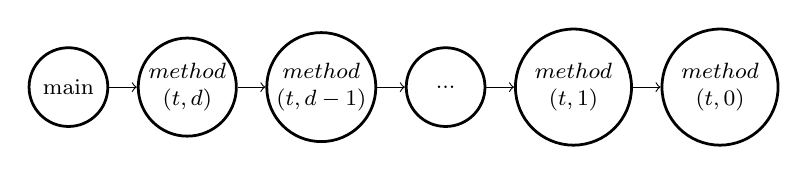
\begin{tikzpicture}[node distance = 1em, auto, font=\footnotesize, align=center, every node/.style={line width=1pt,draw,shape=rectangle,minimum width = 1.0cm}]
    \node (main) [shape=circle]{main};
    \node (c0) [shape=circle, right=of main, inner sep=1pt]{$method$\\$(t, d)$};
    \node (c1) [shape=circle, right=of c0, inner sep=1pt]{$method$\\$(t, d-1)$};
    \node (cp) [shape=circle, right=of c1]{...};
    \node (cn) [shape=circle, right=of cp]{$method$\\$(t,1)$};
    \node (work) [shape=circle, right=of cn]{$method$\\$(t,0)$};  
 
    \draw [->] (main) -- (c0);
    \draw [->] (c0) -- (c1);
    \draw [->] (c1) -- (cp);
    \draw [->] (cp) -- (cn);
    \draw [->] (cn) -- (work);
  \end{tikzpicture}
  \caption{Call Tree of MooBench}
  \label{fig:MooBench}
\end{figure}

\end{document}